\begin{frame}[label = single indices]
    \frametitle{Simulation: single indices}
    \begin{figure}[htbp]
        \centerline{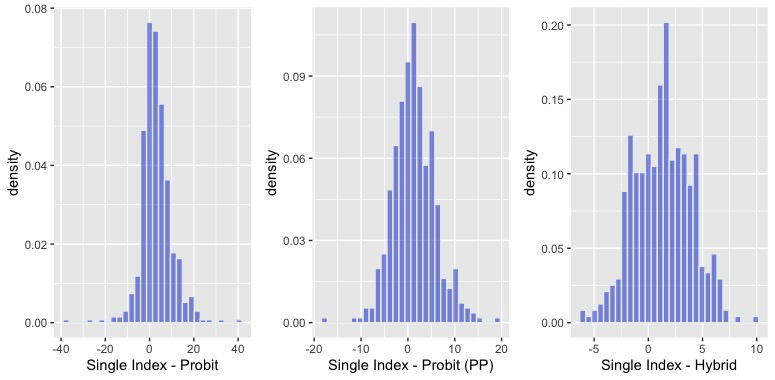
\includegraphics[scale=.35]{content/Figures/Hist_Zij_Design5.png}}
        \caption{\footnotesize{Histogram of $\hat{z}_{12} - z_{12}$ in Design 5}}
        \label{Hist_Zij_Design5}
      \end{figure}
\end{frame}

\begin{frame}
    \frametitle{Simulation: single indices}
    \begin{figure}[htbp]
        \centerline{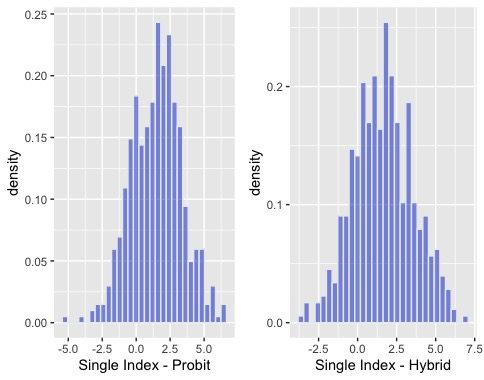
\includegraphics[scale=.35]{content/Figures/Hist_Zij_Design6.png}}
        \caption{\footnotesize{Histogram of $\hat{z}_{12} - z_{12}$ in Design 6}}
        \label{Hist_Zij_Design6}
      \end{figure}
\end{frame}

\begin{frame}
    \frametitle{Simulation: single indices}
    \begin{figure}[htbp]
        \centerline{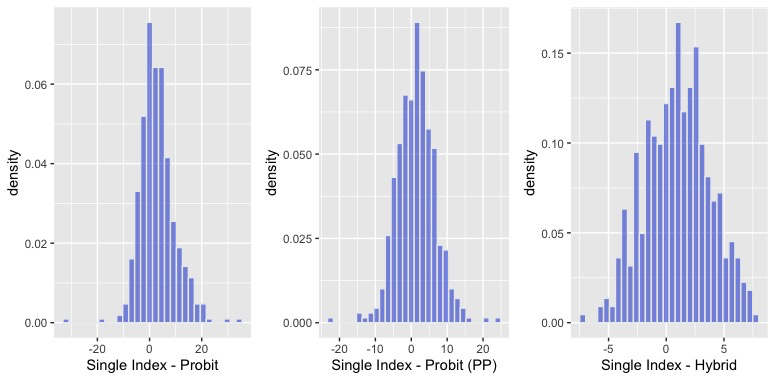
\includegraphics[scale=.35]{content/Figures/Hist_Zij_Design7.png}}
        \caption{\footnotesize{Histogram of $\hat{z}_{12} - z_{12}$ in Design 7}}
        \label{Hist_Zij_Design7}
      \end{figure}
\end{frame}

\begin{frame}
  \frametitle{Simulations: First stage QQ plot for single indices}
  \begin{figure}[htbp]
      \centerline{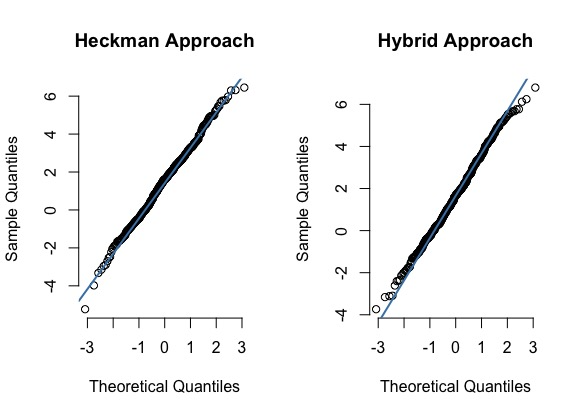
\includegraphics[scale=.35]{content/Figures/QQ_Zij_Design6.png}}
      \caption{\footnotesize{QQ plot of $\hat{z}_{12} - z_{12}$ in Design 6}}
      \label{QQ_Zij_Design6}
    \end{figure}
    With no fixed effects, the distributions are overall well approximated by a normal distribution.
\end{frame}

\begin{frame}
  \frametitle{Simulations: First stage QQ plot for single indices}
  \begin{figure}[htbp]
      \centerline{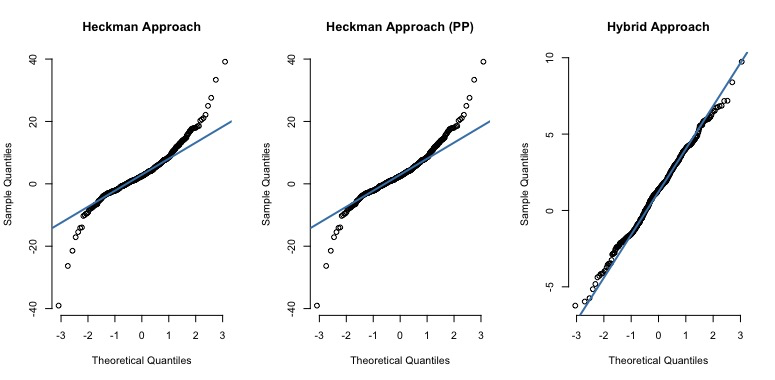
\includegraphics[scale=.35]{content/Figures/QQ_Zij_Design5.png}}
      \caption{\footnotesize{QQ plot of $\hat{z}_{12} - z_{12}$ in Design 5}}
      \label{QQ_Zij_Design5}
    \end{figure}
    In Design 5, the distributions for the Probit and Probit(PP) have heavier tails than the normal distribution $\xrightarrow{}$ mainly affected by the extreme value of fixed effects.
\end{frame}

\begin{frame}
  \frametitle{Simulations: First stage QQ plot for single indices}
  \begin{figure}[htbp]
      \centerline{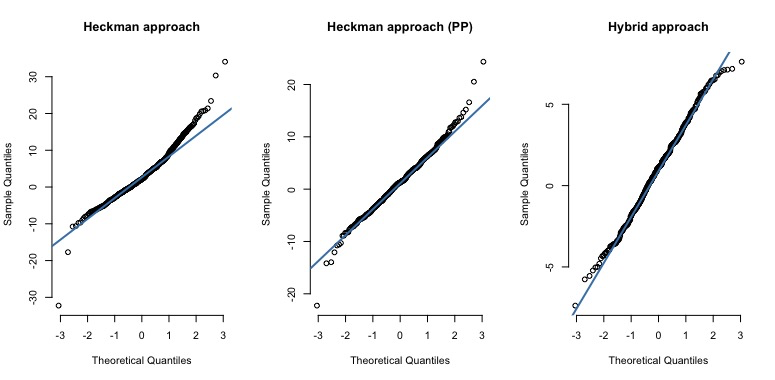
\includegraphics[scale=.35]{content/Figures/QQ_Zij_Design7.png}}
      \caption{\footnotesize{QQ plot of $\hat{z}_{12} - z_{12}$ in Design 7}}
      \label{QQ_Zij_Design7}
    \end{figure}
    In Design 7, the distributions for the Probit and Probit(PP) are more skewed $\xrightarrow{}$ mainly affected by the distribution of the structural parameters.
\end{frame}

\begin{frame}[label = qqplots]
    \frametitle{Simulation: observation equation}
    \begin{figure}[htbp]
        \centerline{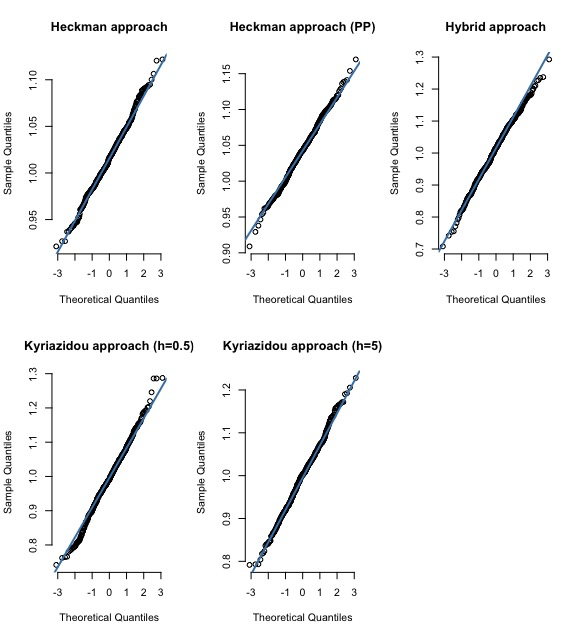
\includegraphics[scale=.3]{content/Figures/QQ_beta_11_Design5.png}}
        \caption{\footnotesize{QQ plot of estimated $\beta_{11}$ in Design 5}}
        \label{QQ_beta_11_Design5}
      \end{figure}
    \end{frame}
      \begin{frame}
        \frametitle{Simulation: observation equation}
      \begin{figure}[htbp]
        \centerline{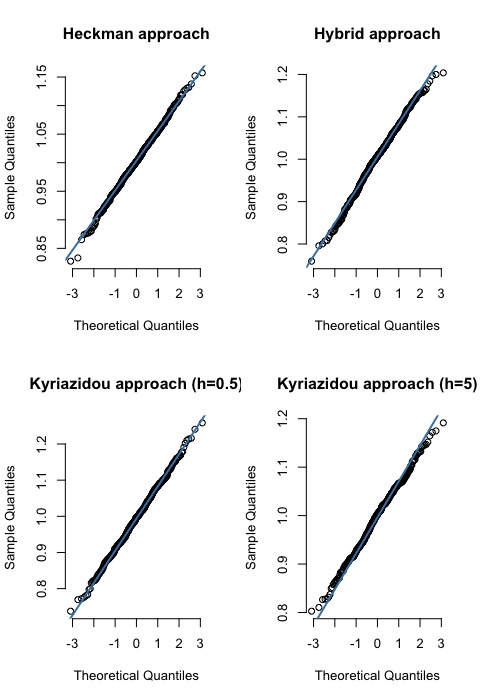
\includegraphics[scale=.3]{content/Figures/QQ_beta_11_Design6.png}}
        \caption{\footnotesize{QQ plot of estimated $\beta_{11}$ in Design 6}}
        \label{QQ_beta_11_Design6}
      \end{figure}
    \end{frame}
      \begin{frame}
        \frametitle{Simulation: observation equation}
      \begin{figure}[htbp]
        \centerline{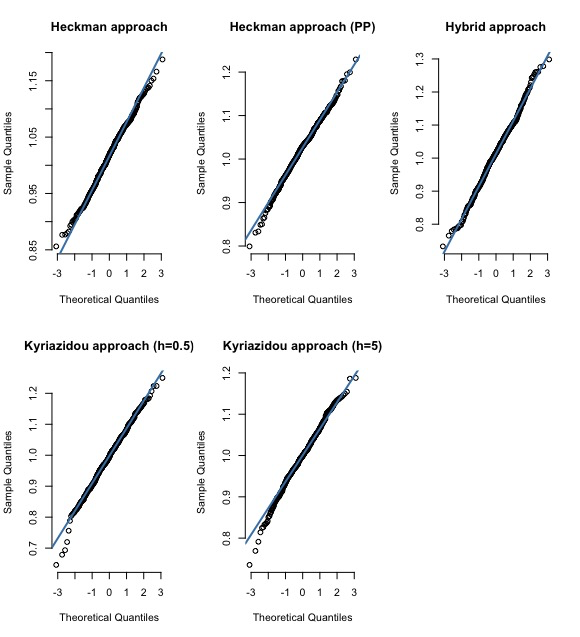
\includegraphics[scale=.3]{content/Figures/QQ_beta_11_Design7.png}}
        \caption{\footnotesize{QQ plot of estimated $\beta_{11}$ in Design 7}}
        \label{QQ_beta_11_Design7}
      \end{figure}
\end{frame}